% $Header: /Users/joseph/Documents/LaTeX/beamer/solutions/conference-talks/conference-ornate-20min.en.tex,v 90e850259b8b 2007/01/28 20:48:30 tantau $
\RequirePackage{filecontents}
\begin{filecontents*}{seminar.bib}
@book{test,
author={John Smith},
title={A book},
publisher={Puplisher},
year={1742},
}
\end{filecontents*}
\documentclass{beamer}
\usepackage{graphicx}
\usepackage{latexsym}		% to get LASY symbols
\usepackage{epsfig}		% to insert PostScript figures
\usepackage{rotating}		% for sideways tables/figures
\usepackage{eufrak}
\usepackage{natbib}
\def\newblock{\hskip .11em plus .33em minus .07em}

% This file is a solution template for:

% - Talk at a conference/colloquium.
% - Talk length is about 20min.
% - Style is ornate.



% Copyright 2004 by Till Tantau <tantau@users.sourceforge.net>.
%
% In principle, this file can be redistributed and/or modified under
% the terms of the GNU Public License, version 2.
%
% However, this file is supposed to be a template to be modified
% for your own needs. For this reason, if you use this file as a
% template and not specifically distribute it as part of a another
% package/program, I grant the extra permission to freely copy and
% modify this file as you see fit and even to delete this copyright
% notice. 


\mode<presentation>
{
  \usetheme{CambridgeUS}
  % or ...

  \setbeamercovered{transparent}
  % or whatever (possibly just delete it)
}

\usepackage[english]{babel}
% or whatever

\usepackage[latin1]{inputenc}
% or whatever

\usepackage{times}
\usepackage[T1]{fontenc}
% Or whatever. Note that the encoding and the font should match. If T1
% does not look nice, try deleting the line with the fontenc.


\title{Easy Deposit} % (optional, use only with long paper titles)

%\subtitle
%{Include Only If Paper Has a Subtitle}

\author[] % (optional, use only with lots of authors)
{MUHAMMED ASHIQU K. (13BCS11104) \\SABEER (13BCS11128)\\SAFEELA NASRIN C. P. (13BCS11130)\\SARANNYA C. (13BCS11133) \\SHAMSEENA N. B. (13BCS11148)}

\institute[MES College of Engineering] % (optional, but mostly needed)
{
 
  \\
  Guide: SREEKESH NAMBOODIRI T.\\
         Assistant Professor\\ 
         Department of Computer Science \& Engineering \\
         MES College of Engineering , Kuttippuram}

% - Use the \inst command only if there are several affiliations.
% - Keep it simple, no one is interested in your street address.

%\date[CFP 2003] % (optional, should be abbreviation of conference name)
%{Conference on Fabulous Presentations, 2003}
% - Either use conference name or its abbreviation.
% - Not really informative to the audience, more for people (including
%   yourself) who are reading the slides online

\subject{Theoretical Computer Science}
% the beginning of each subsection:
\AtBeginSubsection[]
{
  \begin{frame}<beamer>{Outline}
    \tableofcontents[currentsection,currentsubsection]
  \end{frame}
}


% If you wish to uncover everything in a step-wise fashion, uncomment
% the following command: 

%\beamerdefaultoverlayspecification{<+->}


\begin{document}

\begin{frame}
  \titlepage
\end{frame}

%\begin{frame}{Outline}
 % \tableofcontents
  % You might wish to add the option [pausesections]
%\end{frame}


% Structuring a talk is a difficult task and the following structure
% may not be suitable. Here are some rules that apply for this
% solution: 

% - Exactly two or three sections (other than the summary).
% - At *most* three subsections per section.
% - Talk about 30s to 2min per frame. So there should be between about
%   15 and 30 frames, all told.

% - A conference audience is likely to know very little of what you
%   are going to talk about. So *simplify*!
% - In a 20min talk, getting the main ideas across is hard
%   enough. Leave out details, even if it means being less precise than
%   you think necessary.
% - If you omit details that are vital to the proof/implementation,
%   just say so once. Everybody will be happy with that.

\subsection{Introduction}
\begin{frame}{Introduction}
   \begin{itemize}
 \item Smart phones have greatly penetrated the population, and  they can be used to solve many problems.
\item One such problem faced by daily wage workers is their inability to make any savings.
\item We intend to solve this with our project.

 \end{itemize}
 \end{frame}  

\subsection{Abstract}
\begin{frame}{Abstract}
   \begin{itemize}

 \item The idea is to introduce a mechanism for depositing cash in the bank accounts using recharge coupons.
\item The user can buy coupons of various denominations.

 \end{itemize}
 \end{frame}  
 
 
\subsection{Existing System}
\begin{frame}{Existing System}
\begin{itemize}
 \item Cash Deposit Machines are the most common solution.
\item The user may deposit money to their accounts using CDMs.
\item Many banks provides CDM service.
%\item Cash Deposit Machines are not available in all locations.
%\item Whenever they are available they are rushed.
%\item Many people do not know how to use CDMs.


 \end{itemize}
 \end{frame}  

\subsection{Literature Survey}
\begin{frame}{Literature Survey}
\begin{itemize}
\item Generation of Pseudo Random Numbers is required for coupon generator.
\item The system should be resistant to active attacks.
\item In order to do this, select a set of initial Random Number set called feed.
\item Can use Mersenne Twister (MT) algorithm for the same.

%\footnote{\tiny{}}

\end{itemize}

\footnote{\tiny{Mersenne Twister: A 623-Dimensionally Equidistributed Uniform Pseudo-Random Number Generator}}
\end{frame}


\begin{frame}{Literature Survey}
\begin{itemize}
\item Implements SSL protection for RESTful API, in order to avoid Data Hijacking attacks.
\item Security certificates are maintained by Apache HTTPS server for SSL implementation.
\item We use software based Approach.

\end{itemize}

\footnote{\tiny{Inside SSL: Accelerating Secure Transactions}}

\end{frame}


\begin{frame}{Literature Survey}
%\item Design and implementation of voice command using MFCC and HMMs method 
\begin{itemize}
\item The API of backend server is implemented using RESTful API.
\item Uses Node.JS for platform.
\item Application data can be represented in JSON (Javascript Object Notation) format. 

\end{itemize}

\footnote{\tiny{A Resource Oriented Architecture for the Web of Things.}}

\end{frame}



\subsection{System Design}



\begin{frame}{Data Flow Diagram level 1}
\begin{figure}[ht!]
\centering
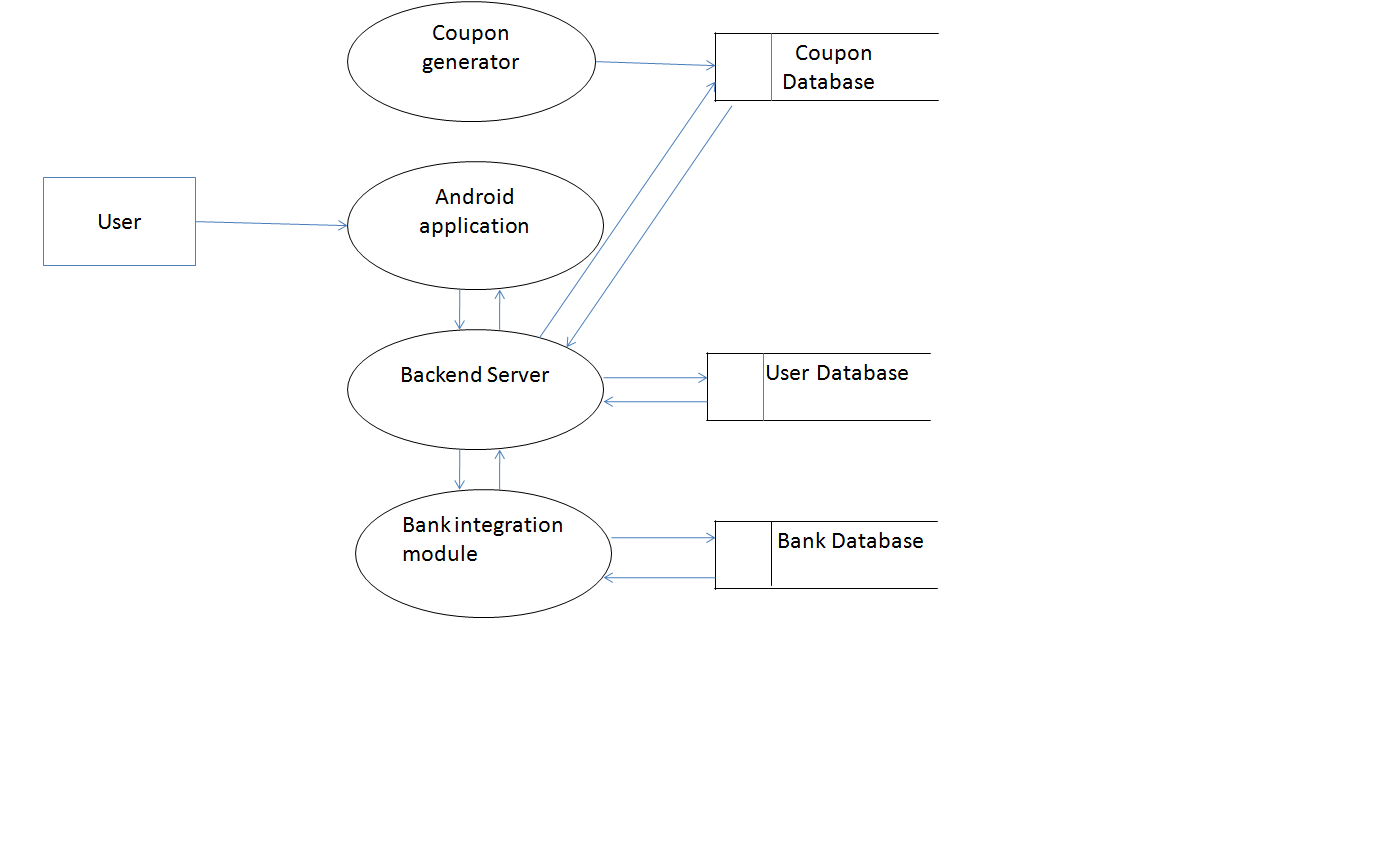
\includegraphics[scale=0.4]{lvl.png}
\end{figure}
\end{frame}

\subsection{Module Description}
\begin{frame}{Module Description}
\item The system consists of 4 modules 
\begin{itemize}
\item Android application
\item Backend Server
\item Coupon generator
\item Bank integration module

\end{itemize}
\end{frame}



\begin{frame}{Android application}
\begin{itemize}
\item The application communicates with the Backend server using REST call.
\item The response from the Backend server to Android application are provided in JSON format.
\end{itemize}
\end{frame}

\begin{frame}{Backend Server}
\begin{itemize}
\item Backend server is used to serve data to the front end applications, such as the Android application.
\item The application provides data and queries the server using REST calls.
\item The Backend server is hosted on a fully equipped cloud infrastructure with secure certificates.
\end{itemize}
\end{frame}

\begin{frame}{Coupon generator}
\begin{itemize}
\item Coupon generator is used to generate unique coupon codes by a descrete algorithm that avoids collision.
\item The coupon generator also connects to the server to save the generated coupons to the data storage.

\end{itemize}
\end{frame}

\begin{frame}{Bank integration module}
\begin{itemize}
\item Bank integration module is the system that is built to mock the working of a bank.
\item This is used to get the information about the users bank account such as their account balance.
\item The backend server contacts this module using REST requests.
 \end{itemize}
\end{frame}

\subsection{Software Tools and Techniques}
\begin{frame}{Hardware Requirements}
\begin{itemize}
\item Server
\begin{itemize}
\item Processor : Any Quad Core ( > 3 GHz) 
\item Memory : 8 GB or higher 
\item Disk : 20 GB or higher

\end{itemize}
\item Android Application 
\begin{itemize}
\item Processor : Any 
\item Memory : 1 GB or higher

\end{itemize}

\end{itemize}
\end{frame}



\begin{frame}{Software Requirements}
\begin{itemize}
\item Android application
\begin{itemize}
\item Android Studio
\end{itemize}

\item Backend server
\begin{itemize}
\item IDE : WebStorm
\item OS  : Ubuntu(Linux)
\end{itemize}

\end{itemize}
\end{frame}



\subsection{Implementation}
\begin{frame}{Server Configuration}
\begin{figure}
	\centering
	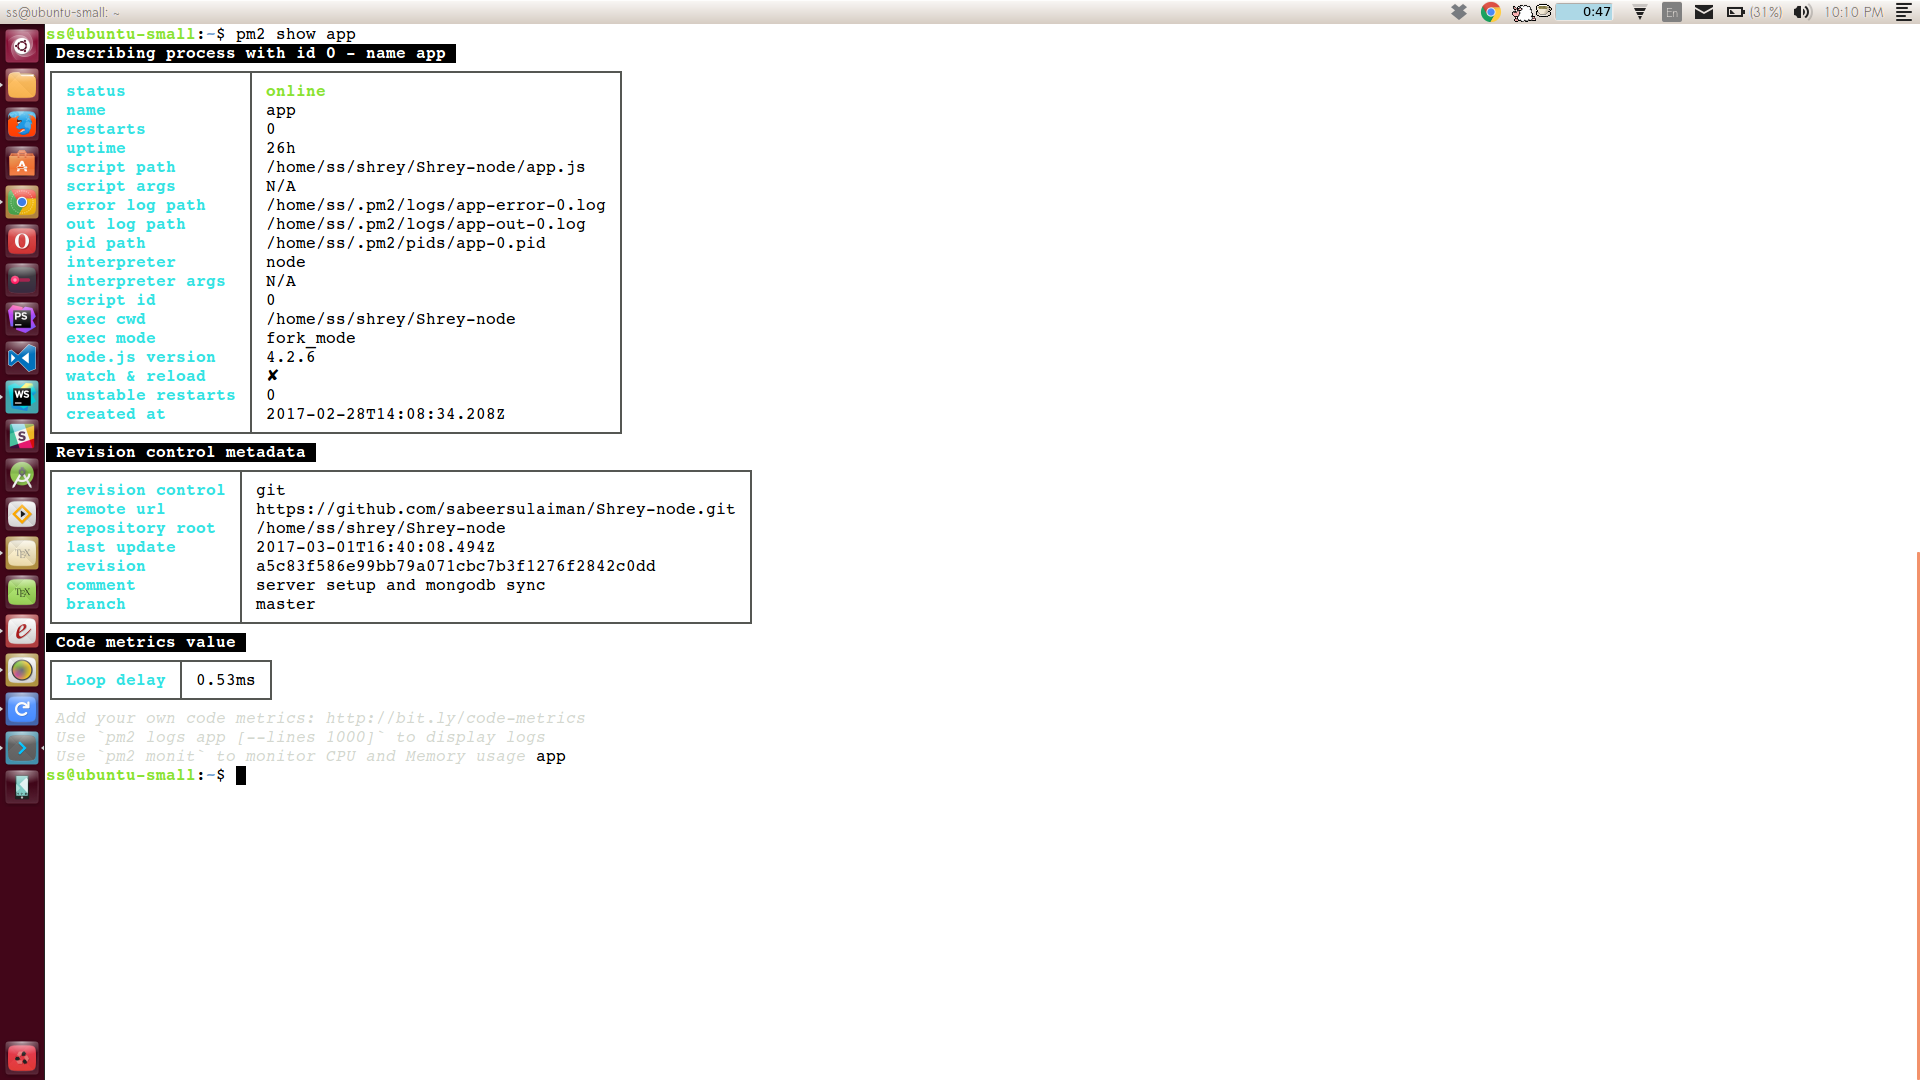
\includegraphics[scale=0.18]{screens/server_screen.png}
\end{figure}
\end{frame}

\begin{frame}{NodeJS Backend}
	\begin{figure}[ht!]
		\centering
		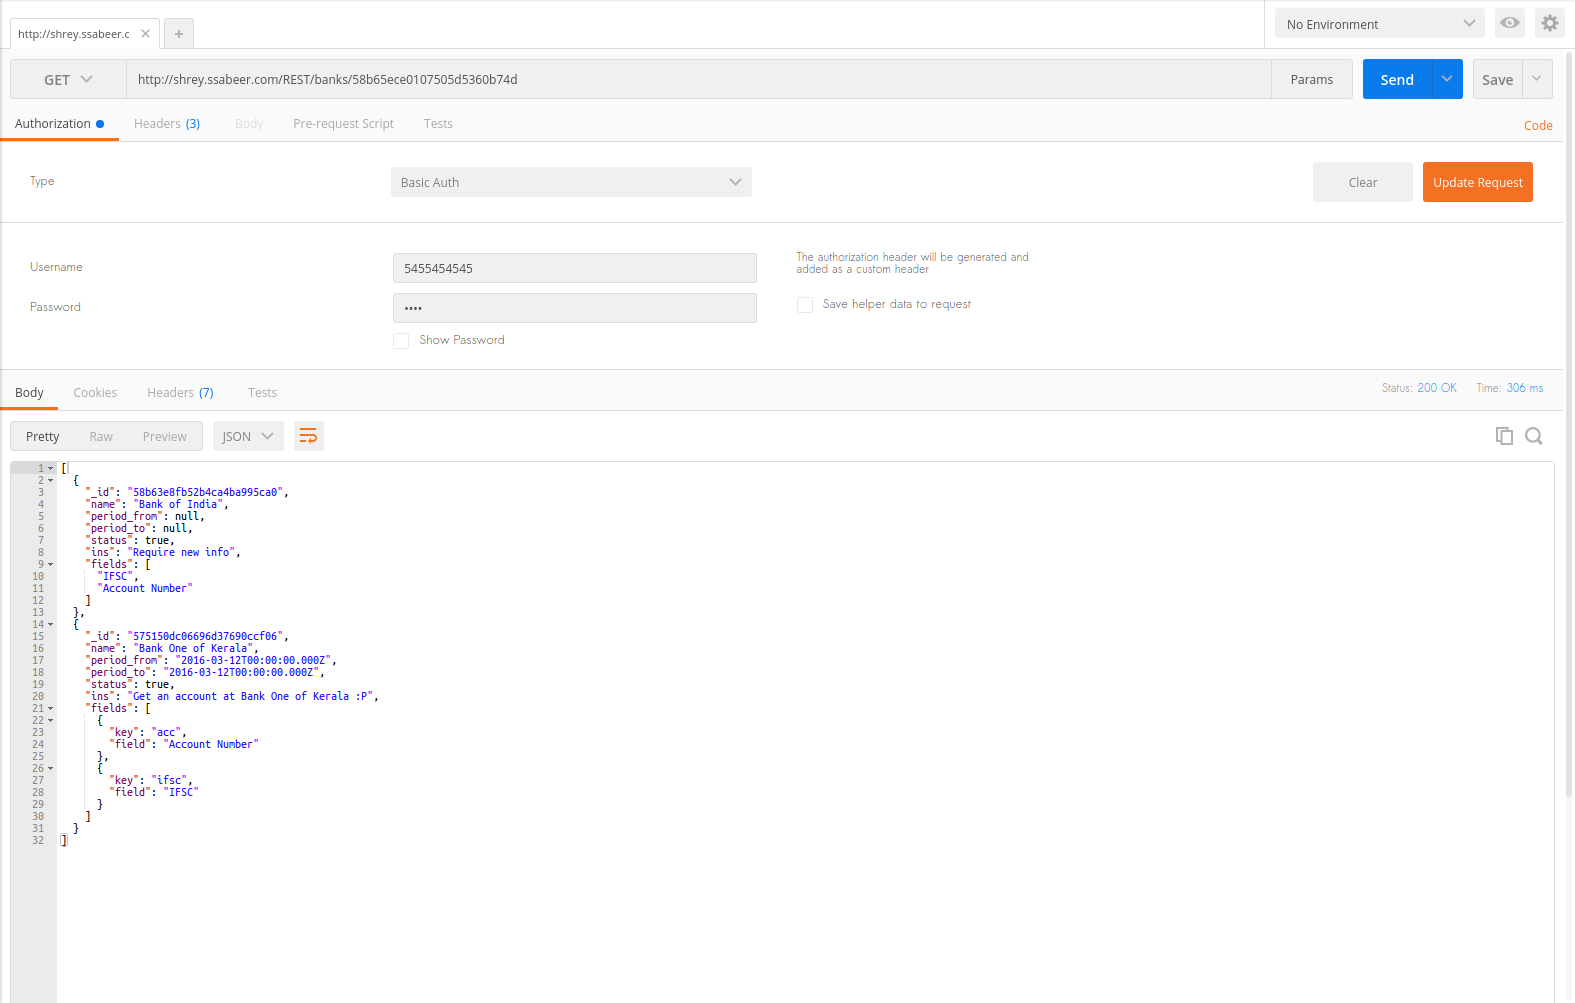
\includegraphics[scale=0.2]{screens/screen_backend_server.png}
	\end{figure}
\end{frame}


\begin{frame}{Android Application}
	\begin{figure}[ht!]
		\centering
		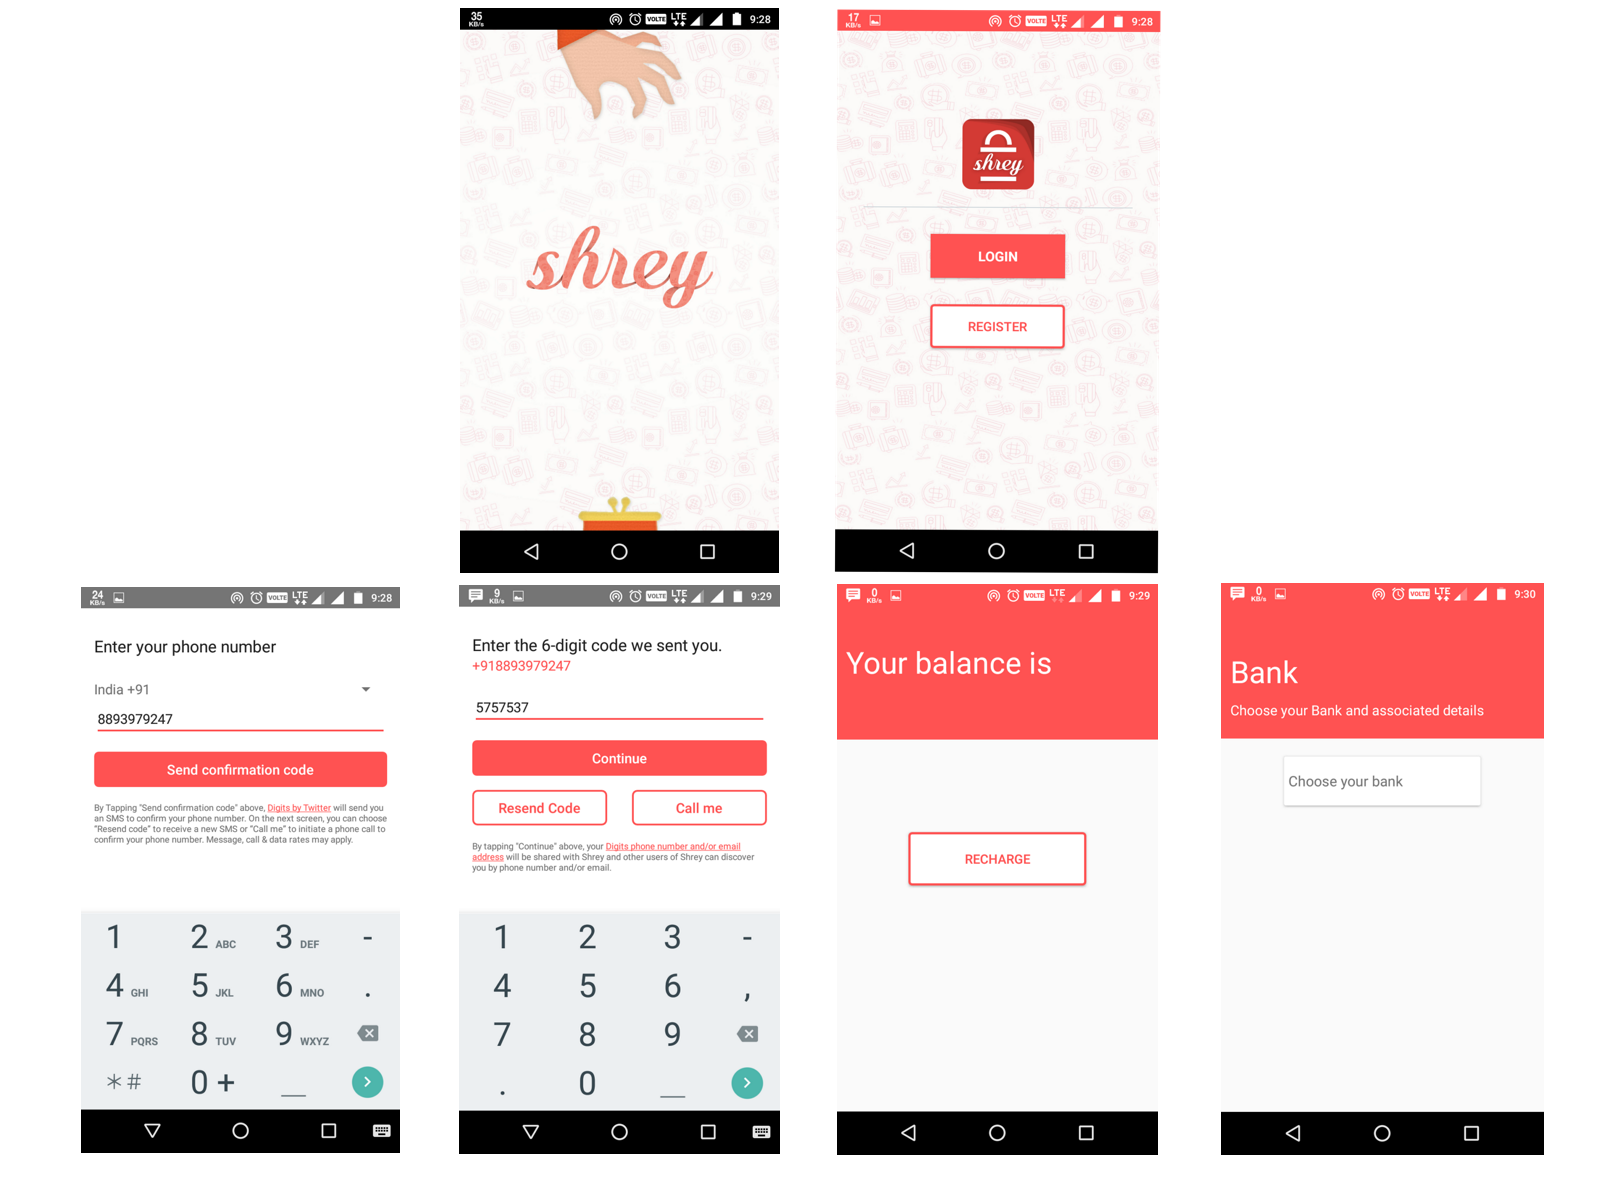
\includegraphics[scale=0.25]{screens/android_screens.png}
	\end{figure}
\end{frame}


 \subsection{Conclusion}
\begin{frame}{Conclusion}
\begin{itemize}
\item Our project will serve as a way to easily deposit money in bank accounts.
\item It�s cloud based architecture will help to accommodate a large amount of users.
\end{itemize}
\end{frame}


 \subsection{References}
\begin{frame}
\frametitle{References}
\footnotesize{
\begin{thebibliography}{99}



\bibitem[Label1, 2011]{key1}[1] Dominique Guinard, Vlad Trifa, Erik Wilde
 \newblock "A Resource Oriented Architecture for the Web of Things ",
 \newblock \emph{ Internet of Things (IOT) Conference, April 2011}.
 

 \bibitem[Label1, 2011]{key2}[2] MAKOTO MATSUMOTO, TAKUJI NISHIMURA 
 \newblock "Mersenne Twister: A 623-Dimensionally Equidistributed Uniform Pseudo-Random Number Generator",
 \newblock \emph{ACM Transactions on Modeling, October 2010 }.
 

\bibitem[Label1, 2011]{key3}[3] Wesley Chou
\newblock "Inside SSL: Accelerating Secure Transactions",
\newblock \emph{ITPro IEEE, September | October 2002}.


% \bibitem[Label1, 2011]{key4}[4] Xufei Mao,Shaojie Tang, Xiahua Xu,
 %\newblock "Energy efficient Oppurtunistic Routing in Wireless Sensor Network
%s",
% \newblock \emph{IEEE transactions on parellel and distributed systems, VOL. 12, NO. 2, February 2011 }

%\bibitem[Label1, 2011]{key5}[5] Tapaliana Bhattasali,Rituparna Chaki,Sugata Sanyal
% \newblock "Sleep Deprivation Attack Detection in Wireless Sensor Networks",
% \newblock \emph{International journal of computer applications(0975-8887)vol 40- No: 15,February 2012 }
 
% \bibitem[Label1, 2011]{key6}[6] Eugene Y. Vasserman, Nicholas Hopper,
% \newblock " Vampire Attacks: Draining Life from Wireless Ad Hoc Sensor Networks",
% \newblock \emph{IEEE transactions on mobile computing, VOL. 12, NO. 2, February 2013 }
 
%  \bibitem[Label1, 2011]{key7}[7] Yazeed Al-Obaisat,Robin Braun,
% \newblock "On Wireless Sensor Networks: Architectures,Protocols,Applications and Management",
% \newblock \emph{Institute of Information and Communication Technologies,May 2004 }
  
\end{thebibliography}
}
\end{frame}

 
\begin{frame}
\centerline{Thank You}
\end{frame}
% End of slides

\end{document}

